% =====================================================================================================
%  Part 3 - IEEE report (two-column, IEEEtran conference template)
%  Build:  latexmk -pdf -interaction=nonstopmode main.tex      (MiKTeX)
%
%  HOW TO USE THIS FILE
%  * Every red [TEAM: ...] box marks a paragraph the authors write IN THEIR OWN WORDS.
%    Each box lists what the paragraph must say and the exact numbers to use (all taken from 2_model/results).
%    outline.md contains the same guidance in more detail. Delete each box once its paragraph is written.
%  * Tables are generated by build_tables.py from the results CSVs - do not edit tables/*.tex by hand.
%  * Equations, figures, tables, captions and references are complete.
%  * Before submitting: no red boxes left; run the ieee-format-checker, results-checker and reference-verifier
%    agents; set \TEAMDRAFTfalse below to hide any leftover boxes (they would then be missing text!).
% =====================================================================================================
\documentclass[conference]{IEEEtran}
\IEEEoverridecommandlockouts

\usepackage{cite}
\usepackage{amsmath,amssymb,amsfonts}
\usepackage{graphicx}
\usepackage{booktabs}
\usepackage{multirow}
\usepackage{xcolor}
\usepackage{url}
\usepackage[hidelinks]{hyperref}

\graphicspath{{figures/}}

% ---- writing placeholders -----------------------------------------------------------------------
\newif\ifTEAMDRAFT \TEAMDRAFTtrue
\newcommand{\TEAM}[1]{\ifTEAMDRAFT{\color{red}\small[\textbf{TEAM:} #1]}\fi}

\begin{document}

% =====================================================================================================
\title{Calibrated Machine-Learning Models for ICU Mortality Prediction on MIMIC-IV: A Case Study in
Leakage-Free Validation and Subgroup Reporting}

\author{
\IEEEauthorblockN{Mudassar}
\IEEEauthorblockA{\textit{\TEAM{Department}} \\
\textit{\TEAM{University}}\\
\TEAM{City, Country} \\
\TEAM{e-mail}}
\and
\IEEEauthorblockN{Touseef}
\IEEEauthorblockA{\textit{\TEAM{Department}} \\
\textit{\TEAM{University}}\\
\TEAM{City, Country} \\
\TEAM{e-mail}}
\and
\IEEEauthorblockN{Ifraz}
\IEEEauthorblockA{\textit{\TEAM{Department}} \\
\textit{\TEAM{University}}\\
\TEAM{City, Country} \\
\TEAM{e-mail}}
}

\maketitle

% =====================================================================================================
\begin{abstract}
\TEAM{150--250 words, one paragraph, no citations. Cover in this order: (1) problem - ICU mortality models are
usually judged by AUROC alone, while calibration, missing-data handling, leakage-free validation and subgroup
performance are rarely reported; (2) what you did - a fixed MIMIC-IV cohort (51,838 first ICU stays, 10.65\%
in-hospital mortality), 40 features from the first 24\,h, patient-grouped train/validation/test split, five models
(logistic regression, random forest, XGBoost, LightGBM, MLP) tuned with Optuna, isotonic recalibration and a SOFA
baseline; (3) main results - final ensemble AUROC 0.892 (95\% CI 0.884--0.900), AUPRC 0.559 (0.527--0.585),
ECE 0.003, calibration slope 1.01; XGBoost beat equally tuned logistic regression by +0.062 AUPRC; all models far
above SOFA (AUROC 0.702); complete-case training lowered AUPRC; largest subgroup gap by age (AUROC 0.833--0.922);
(4) one-sentence conclusion about what this means for reporting practice.}
\end{abstract}

\begin{IEEEkeywords}
intensive care unit, mortality prediction, MIMIC-IV, machine learning, calibration, missing data, model validation,
algorithmic fairness
\end{IEEEkeywords}

% =====================================================================================================
\section{Introduction}
\label{sec:intro}

\TEAM{Paragraph 1 - motivation: why early mortality risk in the ICU matters (triage, resource planning,
family communication); published severity scores such as SOFA \cite{vincent1996sofa} and SAPS~II
\cite{legall1993saps}; machine learning on large open databases, mainly MIMIC \cite{johnson2023mimiciv}.}

\TEAM{Paragraph 2 - the gap (from your review protocol): most published MIMIC models report only discrimination
(AUROC); a risk score is only useful if its probabilities are trustworthy \cite{vancalster2019calibration};
missing-data handling, leakage-free validation and subgroup performance are often not reported; reporting guidance
TRIPOD+AI \cite{collins2024tripodai}. Mention that this case study accompanies your systematic review.}

\TEAM{Paragraph 3 - aim and research questions: build and evaluate a mortality model that applies these practices on
one fixed cohort; list the questions you answer (calibration, missing data, validation design, gain over logistic
regression and over SOFA, subgroups).}

\TEAM{Contributions - write as an itemize list of 3--4 items, e.g. (i) a leakage-free pipeline with
patient-grouped splits and validation-only post-hoc choices; (ii) an equal-tuning comparison of five model families
against logistic regression and SOFA with paired bootstrap tests; (iii) controlled experiments on missing-data
strategies and a temporal hold-out; (iv) calibration and subgroup reporting; code publicly available (GitHub URL).}

% =====================================================================================================
\section{Related Work}
\label{sec:related}

\TEAM{Benchmarks: Harutyunyan et al. \cite{harutyunyan2019multitask} (MIMIC-III benchmark, in-hospital mortality
from 48\,h); Purushotham et al. \cite{purushotham2018benchmarking} (deep learning vs. super learner and scores);
Johnson et al. \cite{johnson2017reproducibility} (the same task gives different results under different cohort
definitions - reproducibility problem). Say in your words what each found and what they did not report.}

\TEAM{ML vs. logistic regression: Christodoulou et al. \cite{christodoulou2019systematic} found no average benefit
of ML over logistic regression when comparisons are fair - motivates our equal-tuning comparison.}

\TEAM{Calibration, missing data and fairness: calibration as the ``Achilles heel'' \cite{vancalster2019calibration}
and neural networks being over-confident \cite{guo2017calibration}; the missing-indicator method
\cite{groenwold2012missing}; algorithmic bias in health \cite{obermeyer2019dissecting}. End with one or two
sentences on how your work differs (all four dimensions on one cohort, with CIs).}

% =====================================================================================================
\section{Dataset and Cohort}
\label{sec:data}

\TEAM{Data source: MIMIC-IV v3.x \cite{johnson2023mimiciv} on PhysioNet \cite{goldberger2000physionet};
de-identified EHR from Beth Israel Deaconess Medical Center (Boston); credentialed access (CITI training, data-use
agreement). Name the tables used (patients, admissions, icustays, chartevents, outputevents, inputevents,
procedureevents).}

\TEAM{Cohort and outcome: adults ($\geq$18), first ICU stay per patient, stay $\geq$24\,h; outcome = in-hospital
death (\texttt{hospital\_expire\_flag}). Walk through Table~\ref{tab:cohort} and Fig.~\ref{fig:cohort}: 94,458 stays
$\rightarrow$ 65,366 first stays $\rightarrow$ 51,838 stays of $\geq$24\,h; 5,522 deaths (10.65\%), class ratio
8.4:1. Explain why first stay only (one stay per patient avoids patient-level leakage).}

\begin{table}[!t]
\caption{Cohort selection and patient-grouped data split}
\label{tab:cohort}
\centering
\footnotesize
\begin{tabular}{@{}lrr@{}}
\toprule
Inclusion step & Stays & Excluded \\
\midrule
All ICU stays & 94,458 & -- \\
First ICU stay per patient & 65,366 & 29,092 \\
Age $\geq$ 18 & 65,366 & -- \\
ICU stay $\geq$ 24 h & 51,838 & 13,528 \\
Outcome available & 51,838 & -- \\
\midrule
Split (patient-grouped) & Stays & Deaths \ (rate) \\
\midrule
Train & 33,176 & 3,535 (10.66\%) \\
Validation & 8,294 & 883 (10.65\%) \\
Test & 10,368 & 1,104 (10.65\%) \\
\bottomrule
\end{tabular}

\end{table}

\begin{figure}[!t]
\centering
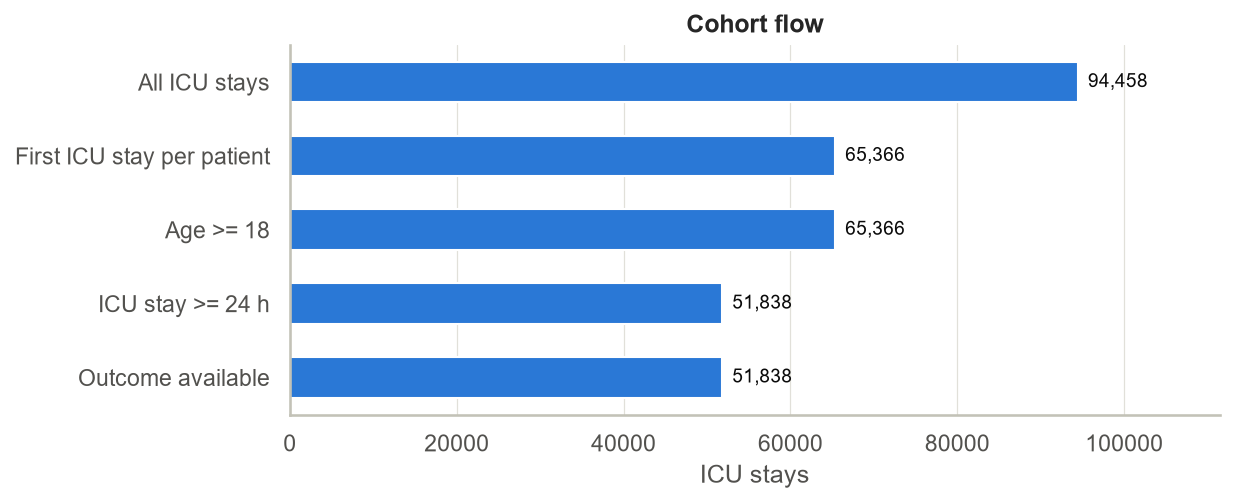
\includegraphics[width=\columnwidth]{fig_cohort_flow.png}
\caption{Cohort selection flow from all MIMIC-IV ICU stays to the analysis cohort.}
\label{fig:cohort}
\end{figure}

\TEAM{Missing data in the cohort: bilirubin, AST, PaCO$_2$ and PaO$_2$ missing in 52--56\% of stays; complete-case
analysis would keep only 13.5\% of stays; missingness is informative - mortality 16.9\% when AST was measured vs.
5.6\% when not (Fig.~\ref{fig:informative}).}

\begin{figure}[!t]
\centering
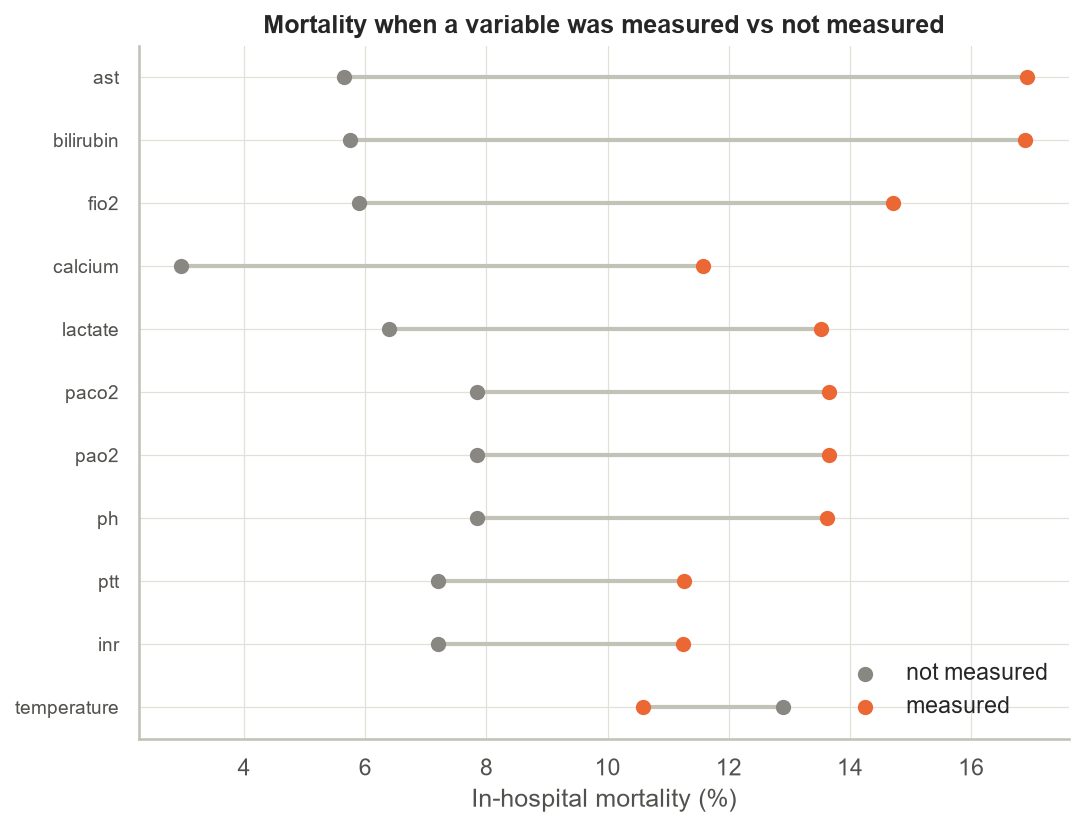
\includegraphics[width=\columnwidth]{fig_informative_missingness.png}
\caption{Mortality by whether a laboratory value was measured in the first 24\,h (informative missingness).}
\label{fig:informative}
\end{figure}

% =====================================================================================================
\section{Methodology}
\label{sec:method}

\subsection{Feature Extraction and Preprocessing}
\TEAM{First-24\,h vitals, GCS, ICU-charted labs, urine output, vasopressors and ventilation; unit harmonisation
(\textdegree F$\rightarrow$\textdegree C, FiO$_2$) and removal of 11,874 physiologically impossible values out of
12.5\,M measurements; mean/min/max/count per variable plus derived features (GCS total, shock index,
PaO$_2$/FiO$_2$, BUN/creatinine). Preprocessing fitted on the training set only: log transform, winsorising, median
imputation with missing-value indicators, one-hot encoding, scaling (257 features). Feature selection on training
data only: near-zero variance, correlation filter ($|r|>0.95$), mutual information + XGBoost importance
$\rightarrow$ 40 features.}

\subsection{Validation Design}
\TEAM{Three patient-grouped, outcome-stratified sets (Table~\ref{tab:cohort}): train 33,176 (64\%), validation
8,294 (16\%), test 10,368 (20\%). Purpose of each set: train = fitting and grouped cross-validation for tuning;
validation = calibration, thresholds, ensemble and final-model choice; test = one final evaluation. State that no
patient appears in two sets (checked in code) and that length of stay, discharge and death dates are never
predictors.}

\subsection{Models and Justification}
\TEAM{Justify each model in one or two sentences: L2 logistic regression (reference model of clinical scores,
interpretable); random forest \cite{breiman2001random} (bagging, non-linear); XGBoost \cite{chen2016xgboost} and
LightGBM \cite{ke2017lightgbm} (gradient boosting, state of the art on tabular data; two libraries to check
robustness); MLP \cite{goodfellow2016deep} (neural approach). Logistic regression vs. XGBoost is the pre-specified
core comparison (hypothesis H3). Implementation with scikit-learn \cite{pedregosa2011scikit}.}

\TEAM{SOFA baseline: computed from worst first-24\,h values for six organ systems \cite{vincent1996sofa}; state the
two deviations (no vasopressor doses, so norepinephrine/epinephrine score 3; missing component = 0); converted to a
probability with a one-variable logistic regression on the training set.}

\subsection{Hyperparameter Tuning}
\TEAM{Optuna with the TPE sampler \cite{akiba2019optuna}, objective = mean AUPRC over 3-fold patient-grouped CV on
the training set; 6--25 trials per model (Table~\ref{tab:tuning}); why AUPRC (imbalanced outcome
\cite{saito2015precision}); class weighting tested separately because it distorts probabilities.}

\subsection{Calibration, Ensemble and Decision Threshold}
\TEAM{Isotonic regression \cite{zadrozny2002transforming} pre-specified and fitted on the validation set; Platt
scaling \cite{platt1999probabilistic} and no calibration reported as sensitivity analysis; scored by 5-fold CV
inside the validation set to get out-of-fold predictions. Ensemble = average of the three best calibrated models by
validation AUPRC, accepted only if $\geq$0.005 AUPRC better than the best single model. Threshold by Youden's
index \cite{youden1950index} on validation data.}

\subsection{Evaluation Metrics}
\TEAM{One or two sentences introducing the metrics, then keep the equations below. Define symbols in your words:
$N$ patients, $y_i\in\{0,1\}$ outcome, $\hat p_i$ predicted risk, $B_m$ the $m$-th of $M=10$ equal-frequency
bins, $p_t$ threshold probability.}

Brier score and expected calibration error (ECE) \cite{guo2017calibration}:
\begin{equation}
\mathrm{Brier}=\frac{1}{N}\sum_{i=1}^{N}\left(\hat p_i-y_i\right)^2,
\label{eq:brier}
\end{equation}
\begin{equation}
\mathrm{ECE}=\sum_{m=1}^{M}\frac{|B_m|}{N}\left|\frac{1}{|B_m|}\sum_{i\in B_m}y_i-\frac{1}{|B_m|}\sum_{i\in B_m}\hat p_i\right|.
\label{eq:ece}
\end{equation}
Calibration slope $\beta$ and intercept $\alpha$ \cite{cox1958two}:
\begin{equation}
\operatorname{logit}P(y_i=1)=\alpha+\beta\,\operatorname{logit}(\hat p_i),
\label{eq:slope}
\end{equation}
where the intercept is estimated with $\beta$ fixed to 1 (calibration-in-the-large). Net benefit for decision-curve
analysis \cite{vickers2006decision}:
\begin{equation}
\mathrm{NB}(p_t)=\frac{\mathrm{TP}(p_t)}{N}-\frac{\mathrm{FP}(p_t)}{N}\cdot\frac{p_t}{1-p_t}.
\label{eq:nb}
\end{equation}

\TEAM{Uncertainty and tests: 95\% percentile-bootstrap CIs with 500 resamples \cite{efron1993introduction}; DeLong
test for correlated AUROCs \cite{delong1988comparing}; paired bootstrap for differences in AUPRC and ECE;
TreeSHAP for explanation \cite{lundberg2017unified,lundberg2020local}; subgroups with fewer than 100 deaths flagged as
unstable.}

\subsection{Protocol Experiments}
\TEAM{(a) Missing-data strategies with logistic regression and XGBoost: imputation + indicator, median imputation
only, complete-case, XGBoost native NaN handling; evaluated on all test stays and on the complete-case subset.
(b) Temporal hold-out: train on 2008--2019 admission periods, test on 2020--2022 (\texttt{anchor\_year\_group});
explain why this is only a weak temporal test (dates shifted per patient).}

% =====================================================================================================
\section{Experimental Setup}
\label{sec:setup}

\TEAM{Software: Python 3.14, scikit-learn 1.8, XGBoost 3.4, LightGBM 4.7, Optuna 5.1, pandas 3.0. Hardware:
8-core CPU, 32\,GB RAM, no GPU; Part~2 runtime about 35\,min. Random seed 42 everywhere. Code and executed notebooks
on GitHub (give URL in a footnote or in the Conclusion). Search spaces: refer to the notebook; summarise trials and
tuning gain with Table~\ref{tab:tuning}.}

\begin{table}[!t]
\caption{Hyperparameter tuning: cross-validated AUPRC with default and tuned settings}
\label{tab:tuning}
\centering
\footnotesize
\begin{tabular}{@{}lrrrr@{}}
\toprule
Model & Trials & Default & Tuned & Gain \\
\midrule
Logistic regression & 15 & 0.505 & 0.505 & $+0.000$ \\
Random forest & 8 & 0.537 & 0.539 & $+0.002$ \\
XGBoost & 25 & 0.535 & 0.560 & $+0.025$ \\
LightGBM & 20 & 0.535 & 0.558 & $+0.023$ \\
MLP & 6 & 0.538 & 0.543 & $+0.005$ \\
\bottomrule
\end{tabular}

\end{table}

% =====================================================================================================
\section{Results}
\label{sec:results}

\subsection{Overall Performance}
\TEAM{Describe Table~\ref{tab:results} and Fig.~\ref{fig:rocpr}: final ensemble (XGBoost + LightGBM + MLP)
AUROC 0.892 (0.884--0.900), AUPRC 0.559 (0.527--0.585) against a prevalence of 0.106; boosted models and MLP close
behind (AUROC 0.888--0.890); logistic regression AUROC 0.869, AUPRC 0.471; SOFA AUROC 0.702, AUPRC 0.229. At the
Youden threshold (0.125): sensitivity 0.822, specificity 0.800, PPV 0.329. DeLong: ensemble AUROC significantly
higher than every other model ($p<0.05$).}

\begin{table*}[!t]
\caption{Test-set performance (10,368 stays) with 95\% bootstrap confidence intervals}
\label{tab:results}
\centering
\scriptsize
\setlength{\tabcolsep}{3.5pt}
\begin{tabular}{@{}lccccccc@{}}
\toprule
Model & AUROC & AUPRC & Brier & ECE & Cal.\ slope & Sensitivity & Specificity \\
\midrule
\textbf{Ensemble (final)} & 0.892 (0.884--0.900) & 0.559 (0.527--0.585) & 0.066 (0.063--0.069) & 0.003 (0.003--0.009) & 1.014 (0.964--1.068) & 0.822 (0.801--0.843) & 0.800 (0.792--0.809) \\
XGBoost & 0.890 (0.882--0.898) & 0.534 (0.503--0.560) & 0.066 (0.063--0.070) & 0.002 (0.003--0.009) & 0.958 (0.907--1.010) & 0.860 (0.839--0.880) & 0.765 (0.756--0.773) \\
LightGBM & 0.889 (0.881--0.897) & 0.533 (0.502--0.560) & 0.067 (0.063--0.070) & 0.004 (0.003--0.010) & 0.965 (0.913--1.017) & 0.841 (0.819--0.864) & 0.783 (0.774--0.792) \\
MLP & 0.888 (0.879--0.896) & 0.520 (0.490--0.546) & 0.067 (0.064--0.070) & 0.004 (0.003--0.010) & 0.979 (0.929--1.028) & 0.843 (0.822--0.866) & 0.776 (0.768--0.784) \\
Random forest & 0.882 (0.872--0.891) & 0.521 (0.490--0.548) & 0.068 (0.064--0.071) & 0.005 (0.003--0.010) & 0.976 (0.926--1.027) & 0.801 (0.777--0.824) & 0.797 (0.789--0.805) \\
Logistic regression & 0.869 (0.859--0.878) & 0.471 (0.443--0.498) & 0.071 (0.068--0.074) & 0.006 (0.004--0.011) & 0.957 (0.907--1.008) & 0.806 (0.785--0.831) & 0.786 (0.778--0.794) \\
SOFA score & 0.702 (0.687--0.717) & 0.229 (0.209--0.250) & 0.088 (0.084--0.092) & 0.004 (0.003--0.011) & 0.974 (0.896--1.060) & 0.825 (0.801--0.846) & 0.472 (0.463--0.483) \\
\bottomrule
\end{tabular}

\end{table*}

\begin{figure*}[!t]
\centering
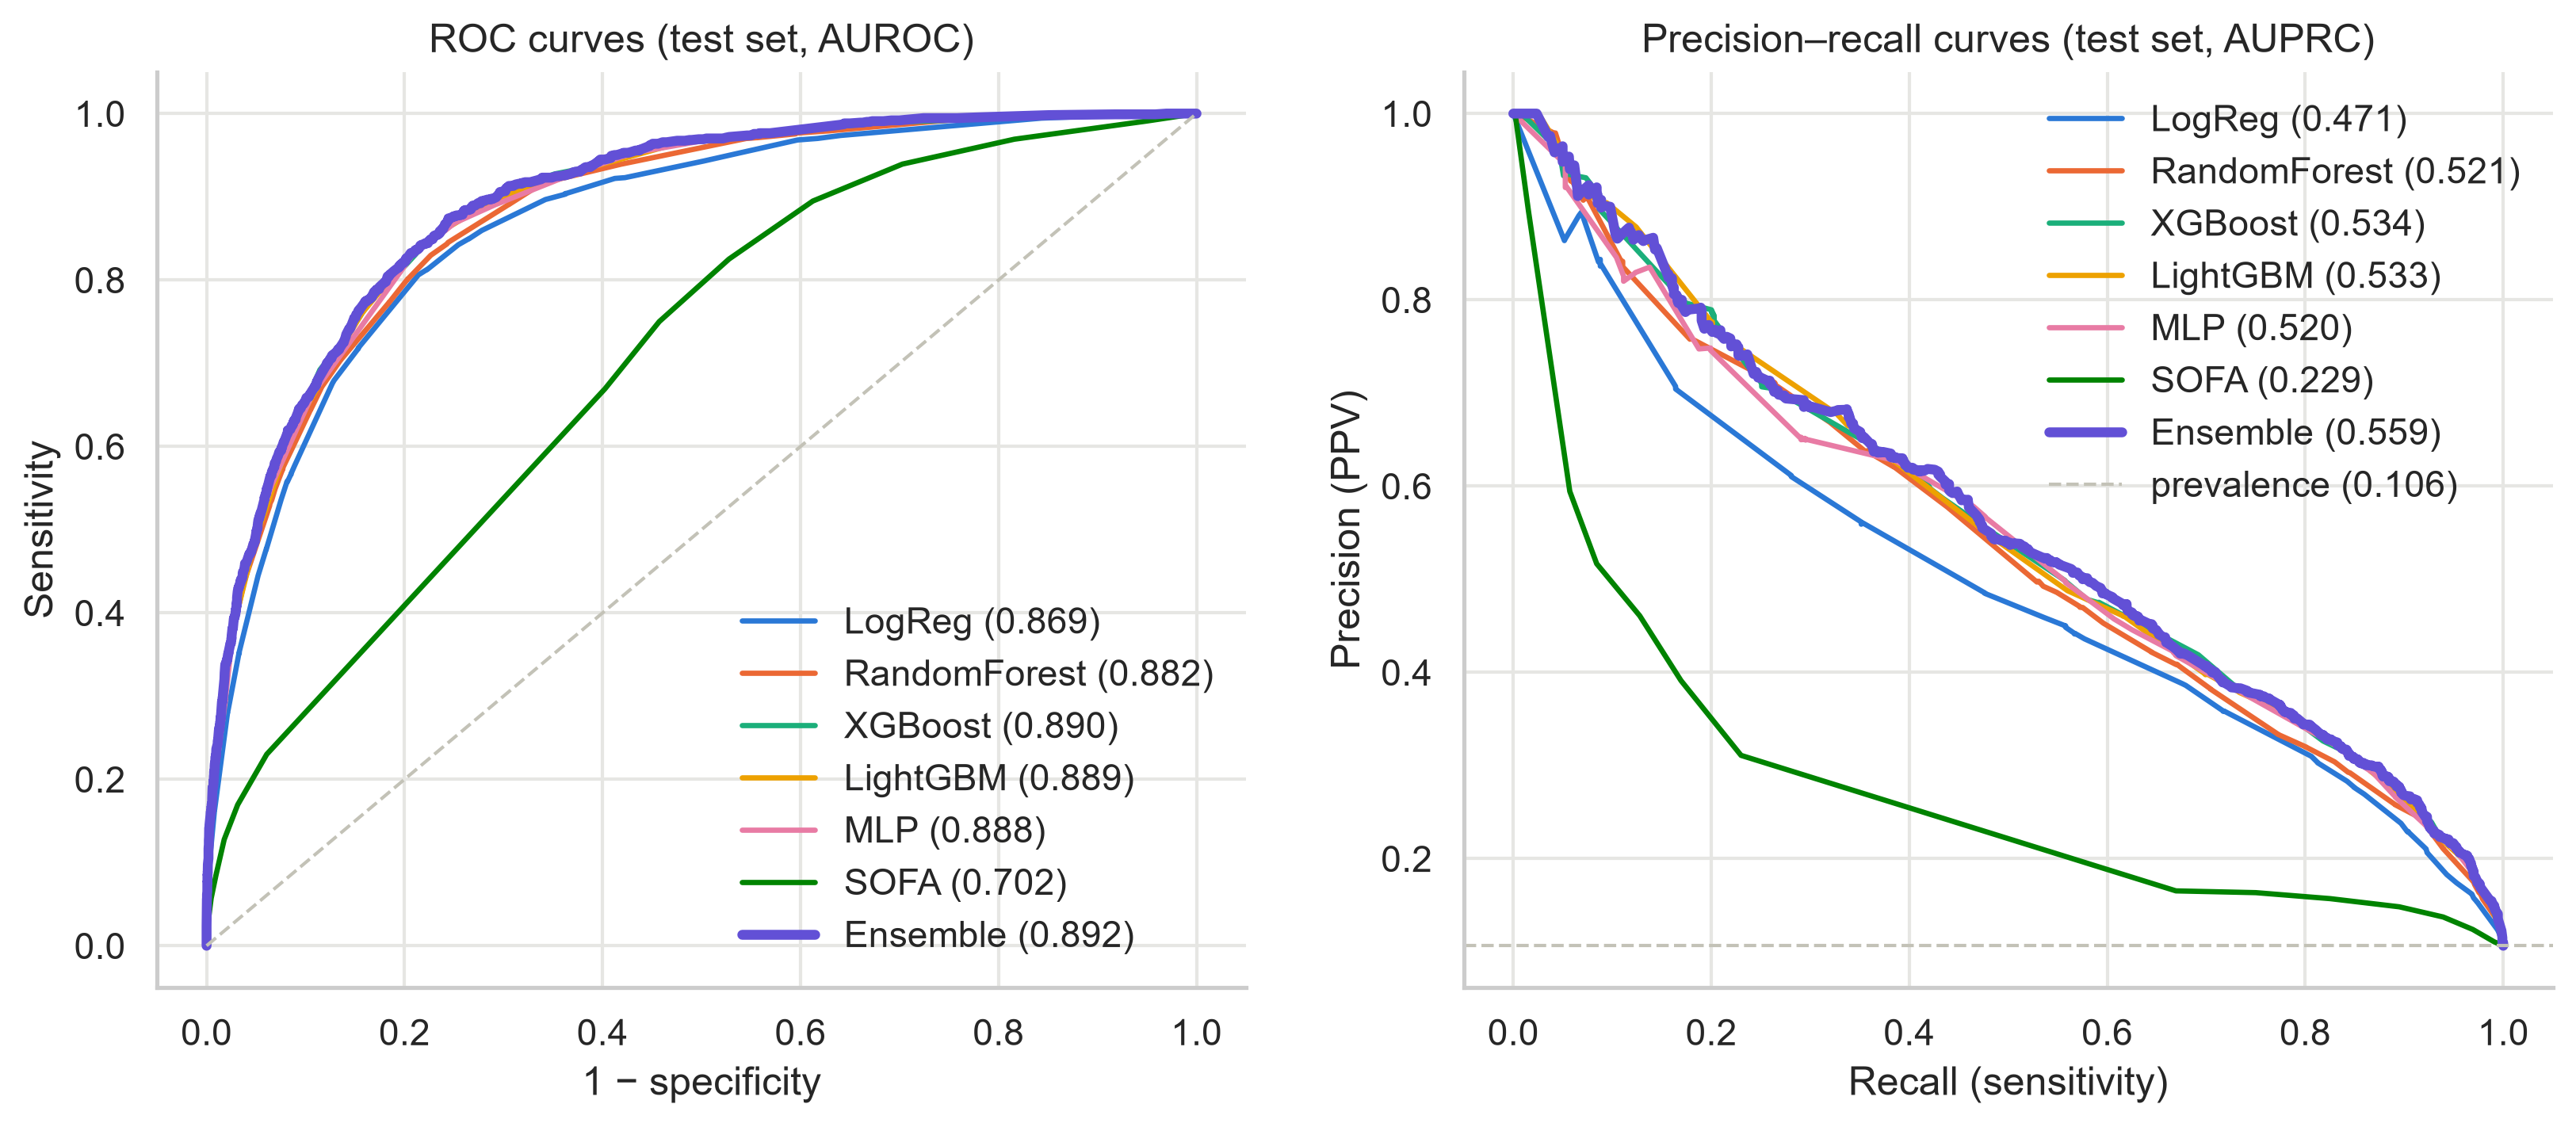
\includegraphics[width=0.8\textwidth]{fig_roc_pr.png}
\caption{ROC (left) and precision--recall (right) curves on the test set; the dashed line in the right panel is the
outcome prevalence.}
\label{fig:rocpr}
\end{figure*}

\subsection{Calibration}
\TEAM{Table~\ref{tab:calib} and Fig.~\ref{fig:calib}: after isotonic recalibration every model has ECE $\leq$0.006 and
a calibration slope between 0.96 and 1.01; final model slope 1.014 (0.964--1.068), intercept 0.011. Compare raw and
recalibrated values from the table and comment on which models needed recalibration most. Class weighting changed
ranking little but pushed predicted risk above observed mortality (from 2\_model/results/val\_class\_weighting.csv).}

\begin{table}[!t]
\caption{Test-set calibration before and after isotonic recalibration}
\label{tab:calib}
\centering
\footnotesize
\begin{tabular}{@{}lrrrr@{}}
\toprule
 & \multicolumn{2}{c}{ECE} & \multicolumn{2}{c}{Cal.\ slope} \\
\cmidrule(lr){2-3}\cmidrule(lr){4-5}
Model & Raw & Isotonic & Raw & Isotonic \\
\midrule
Logistic regression & 0.0118 & 0.0057 & 0.97 & 0.96 \\
Random forest & 0.0090 & 0.0046 & 1.12 & 0.98 \\
XGBoost & 0.0073 & 0.0020 & 1.05 & 0.96 \\
LightGBM & 0.0061 & 0.0041 & 1.01 & 0.97 \\
MLP & 0.0115 & 0.0039 & 0.89 & 0.98 \\
\bottomrule
\end{tabular}

\end{table}

\begin{figure*}[!t]
\centering
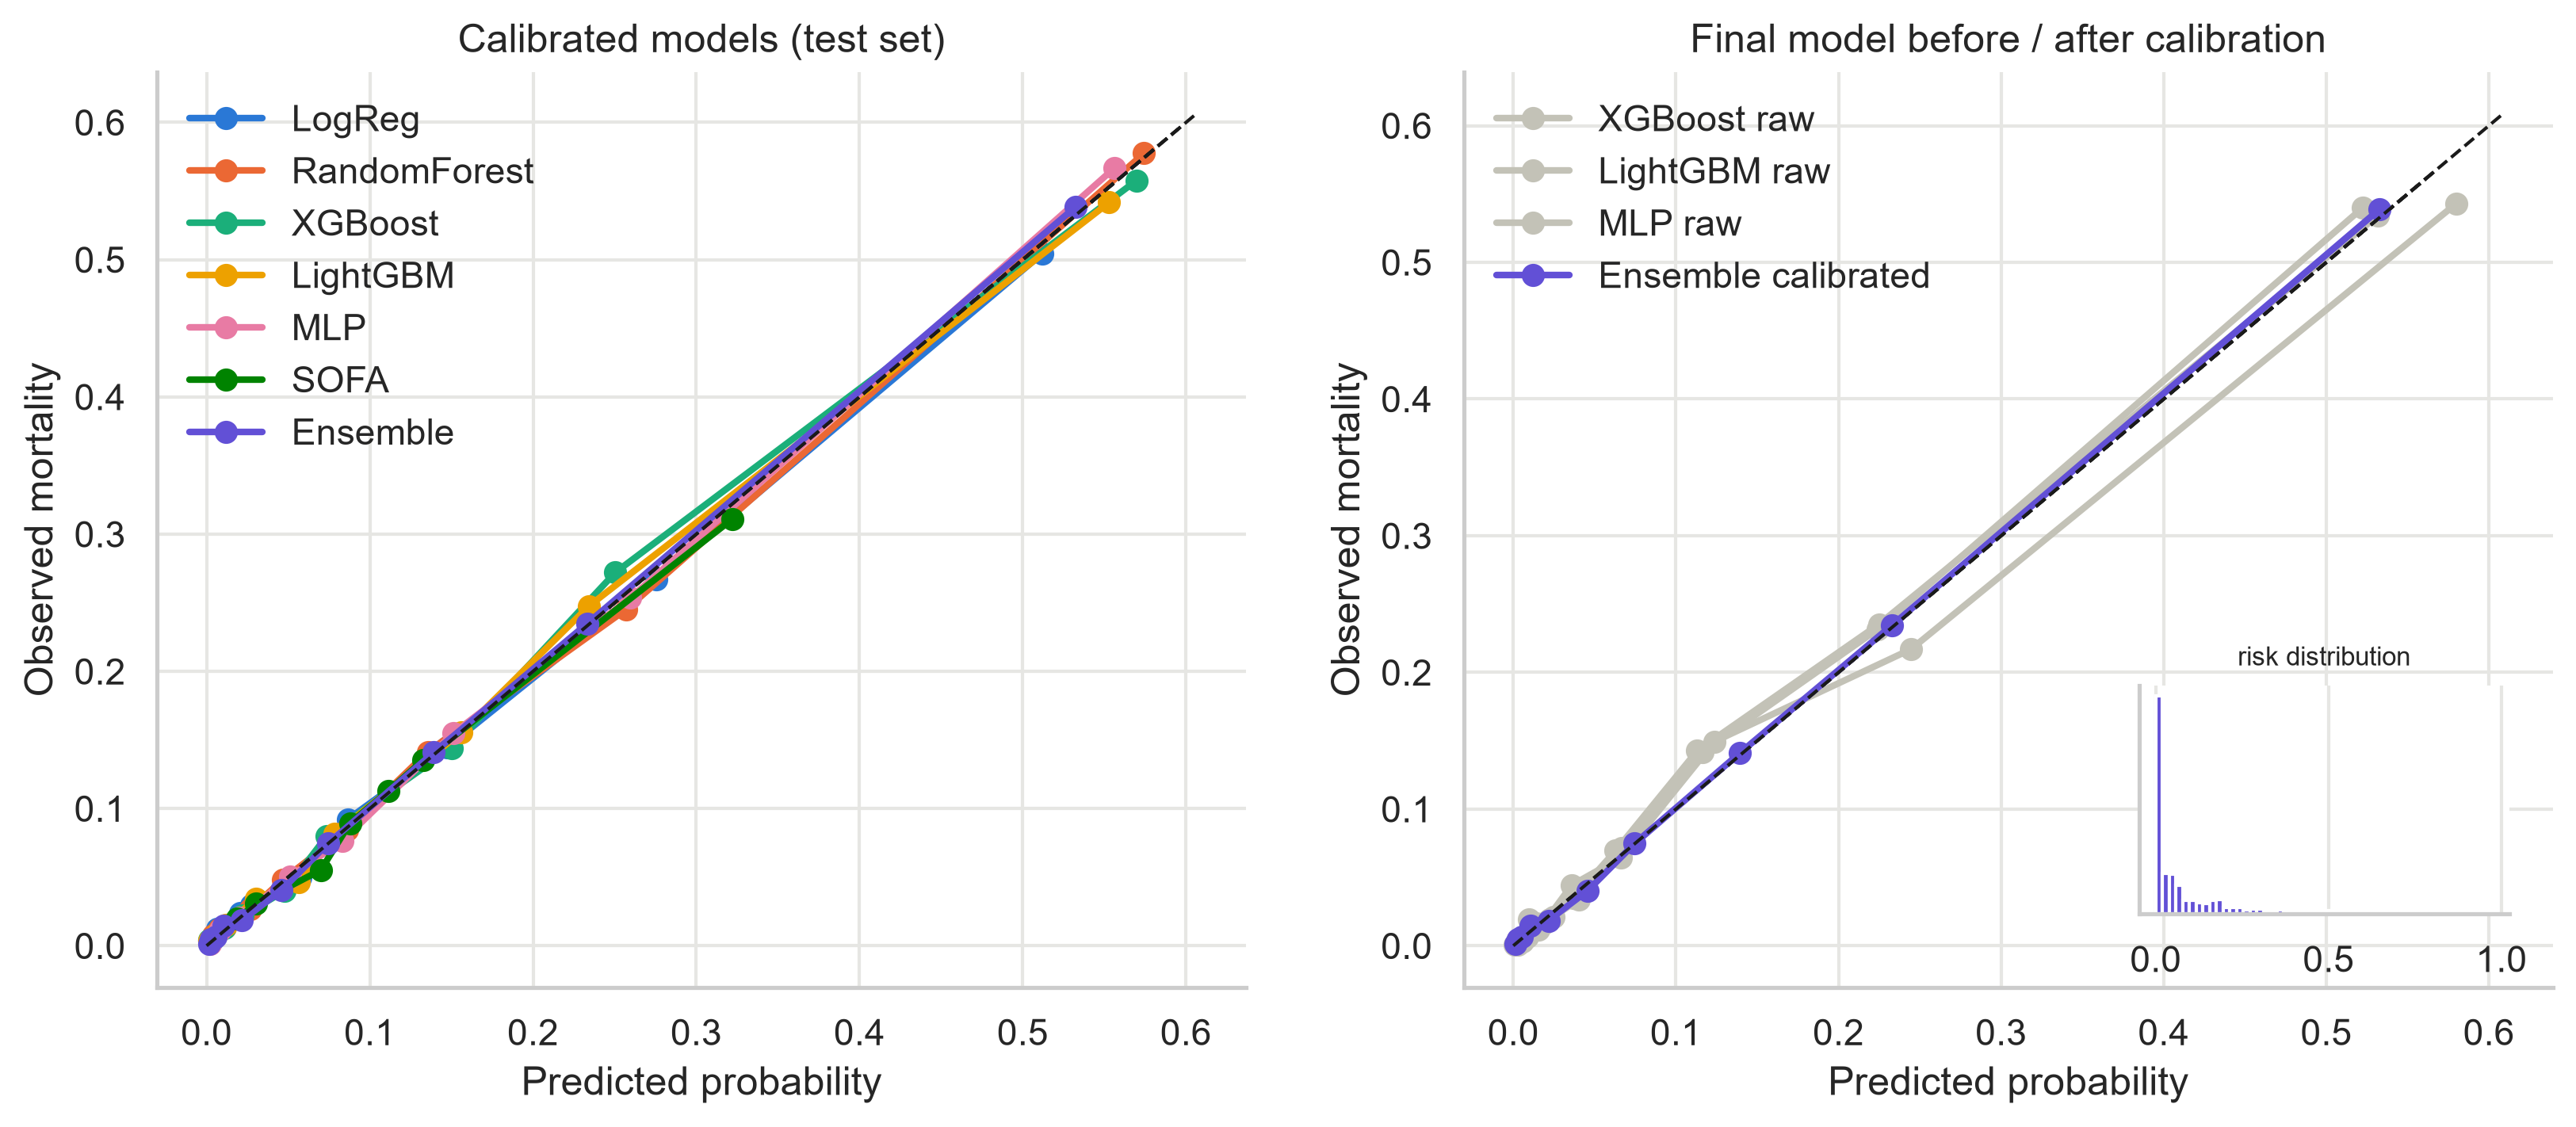
\includegraphics[width=0.8\textwidth]{fig_calibration.png}
\caption{Reliability curves on the test set (10 equal-frequency bins): all calibrated models (left) and the final
model before and after recalibration with its risk distribution (right).}
\label{fig:calib}
\end{figure*}

\subsection{Machine Learning vs. Logistic Regression and SOFA}
\TEAM{Table~\ref{tab:paired} and Fig.~\ref{fig:paired}: XGBoost $-$ logistic regression = +0.062 AUPRC (95\% CI
0.049 to 0.078), ECE difference not significant; ensemble $-$ logistic regression +0.087; logistic regression $-$
SOFA +0.242; ensemble $-$ SOFA +0.330. Interpret against H3: a clear but moderate gain.}

\begin{table}[!t]
\caption{Paired bootstrap differences on the test set}
\label{tab:paired}
\centering
\footnotesize
\begin{tabular}{@{}llrr@{}}
\toprule
Comparison (A $-$ B) & Metric & $\Delta$ & 95\% CI \\
\midrule
XGBoost $-$ LogReg & AUPRC & $+0.062$ & $[+0.049,\ +0.078]$ \\
XGBoost $-$ LogReg & ECE & $-0.004$ & $[-0.006,\ +0.003]$ \\
Ensemble $-$ LogReg & AUPRC & $+0.087$ & $[+0.073,\ +0.103]$ \\
Ensemble $-$ LogReg & ECE & $-0.003$ & $[-0.006,\ +0.004]$ \\
Ensemble $-$ SOFA & AUPRC & $+0.330$ & $[+0.304,\ +0.354]$ \\
Ensemble $-$ SOFA & ECE & $-0.001$ & $[-0.006,\ +0.004]$ \\
LogReg $-$ SOFA & AUPRC & $+0.242$ & $[+0.216,\ +0.263]$ \\
LogReg $-$ SOFA & ECE & $+0.002$ & $[-0.005,\ +0.006]$ \\
\bottomrule
\end{tabular}

\end{table}

\begin{figure*}[!t]
\centering
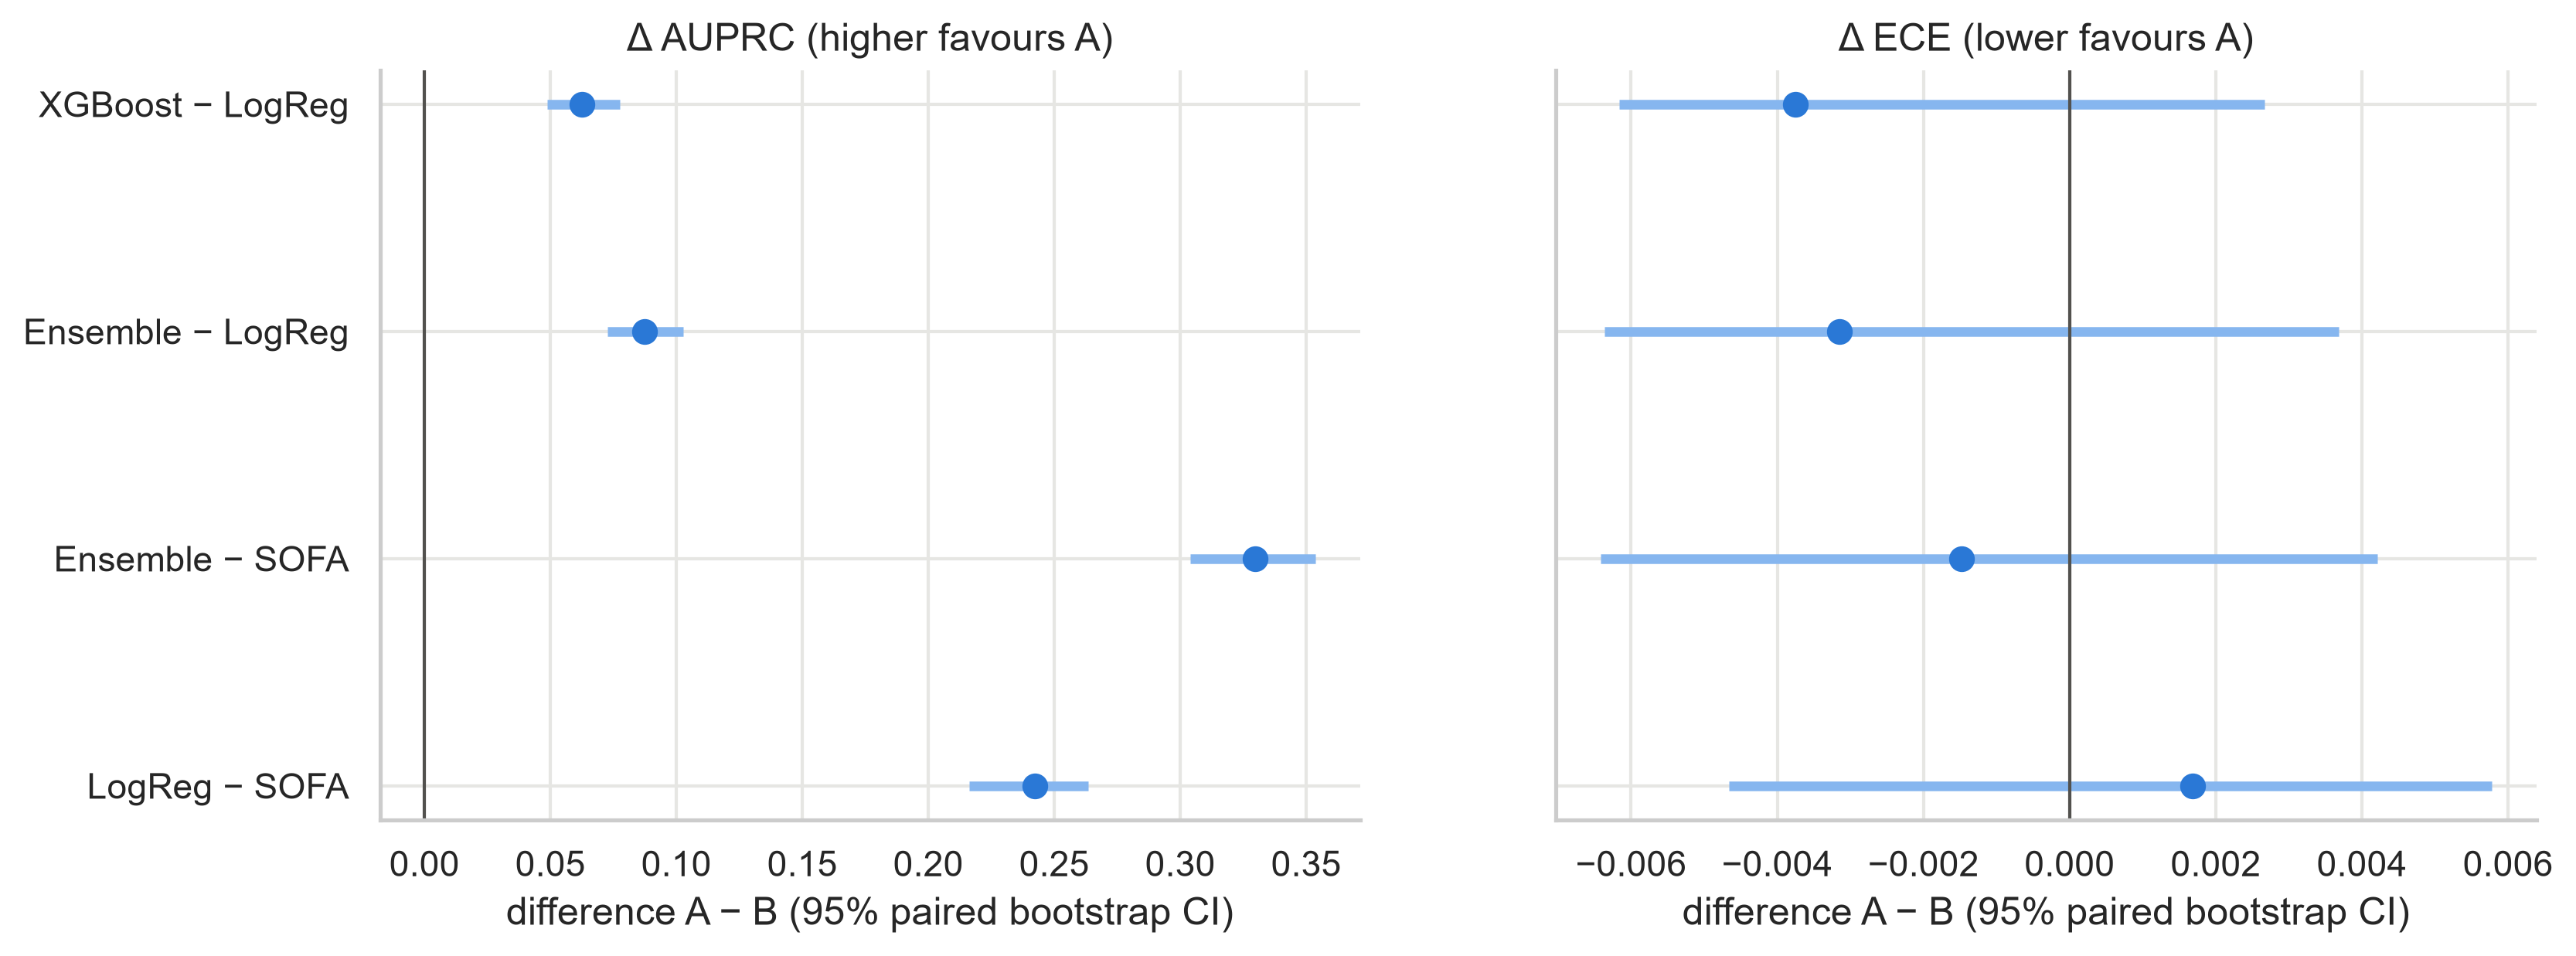
\includegraphics[width=0.78\textwidth]{fig_paired_bootstrap.png}
\caption{Paired bootstrap differences in AUPRC and ECE with 95\% confidence intervals.}
\label{fig:paired}
\end{figure*}

\subsection{Clinical Utility and Explainability}
\TEAM{Fig.~\ref{fig:dca}: net benefit of the final model is above treat-all and treat-none over the threshold range
(describe what you see, compare with logistic regression and SOFA). Fig.~\ref{fig:shap}: most influential features
(read the top ones from the figure: urine output, BUN, respiratory rate, GCS components, ...) and whether their
direction is clinically plausible.}

\begin{figure}[!t]
\centering
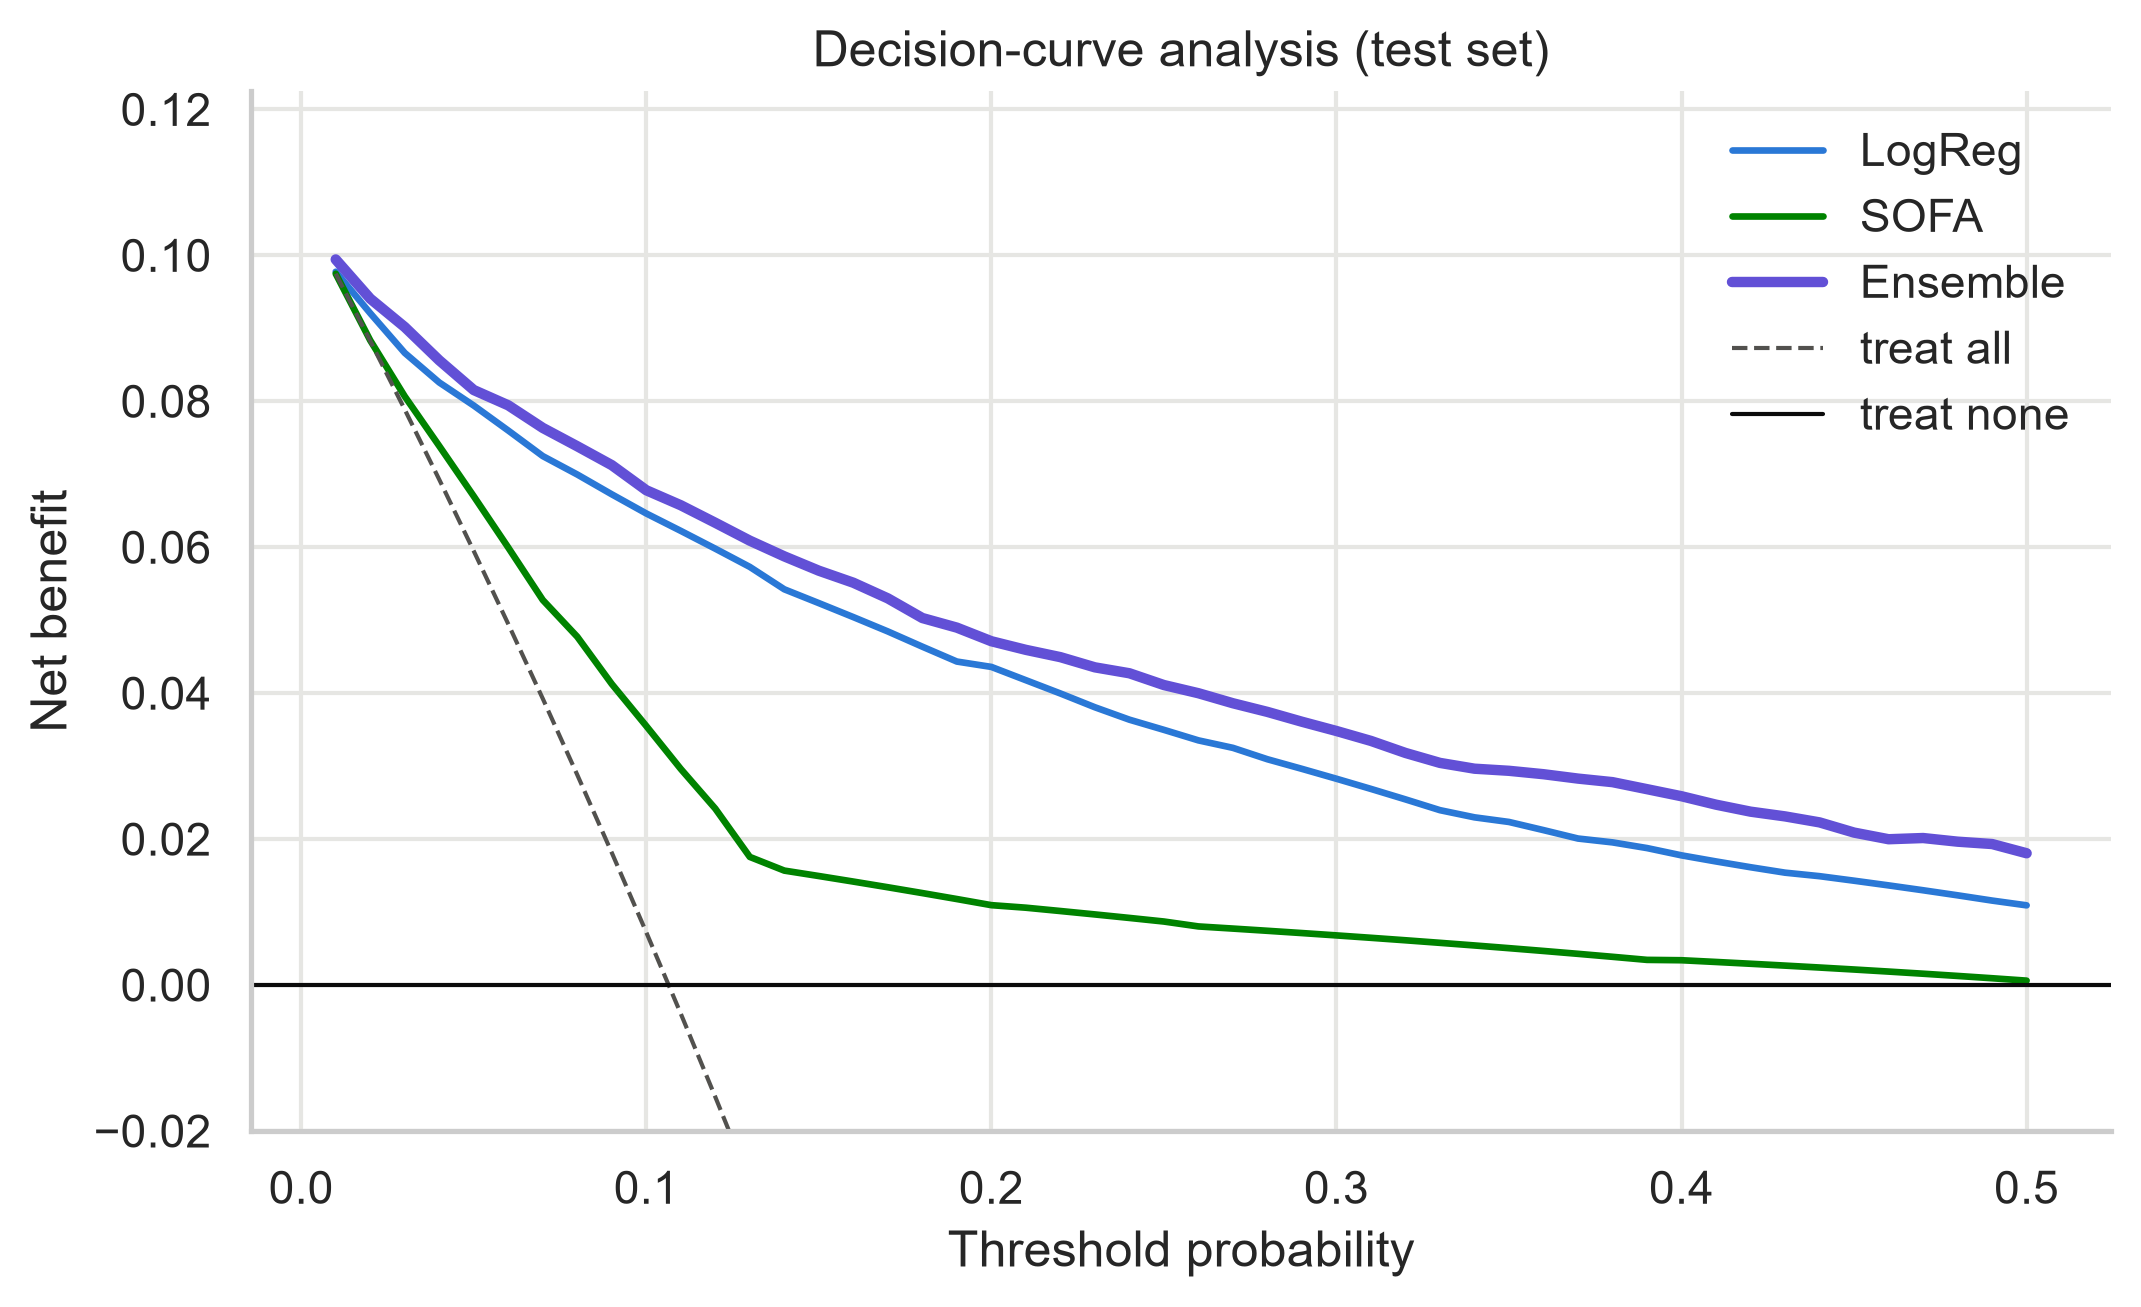
\includegraphics[width=\columnwidth]{fig_decision_curve.png}
\caption{Decision-curve analysis on the test set.}
\label{fig:dca}
\end{figure}

\begin{figure*}[!t]
\centering
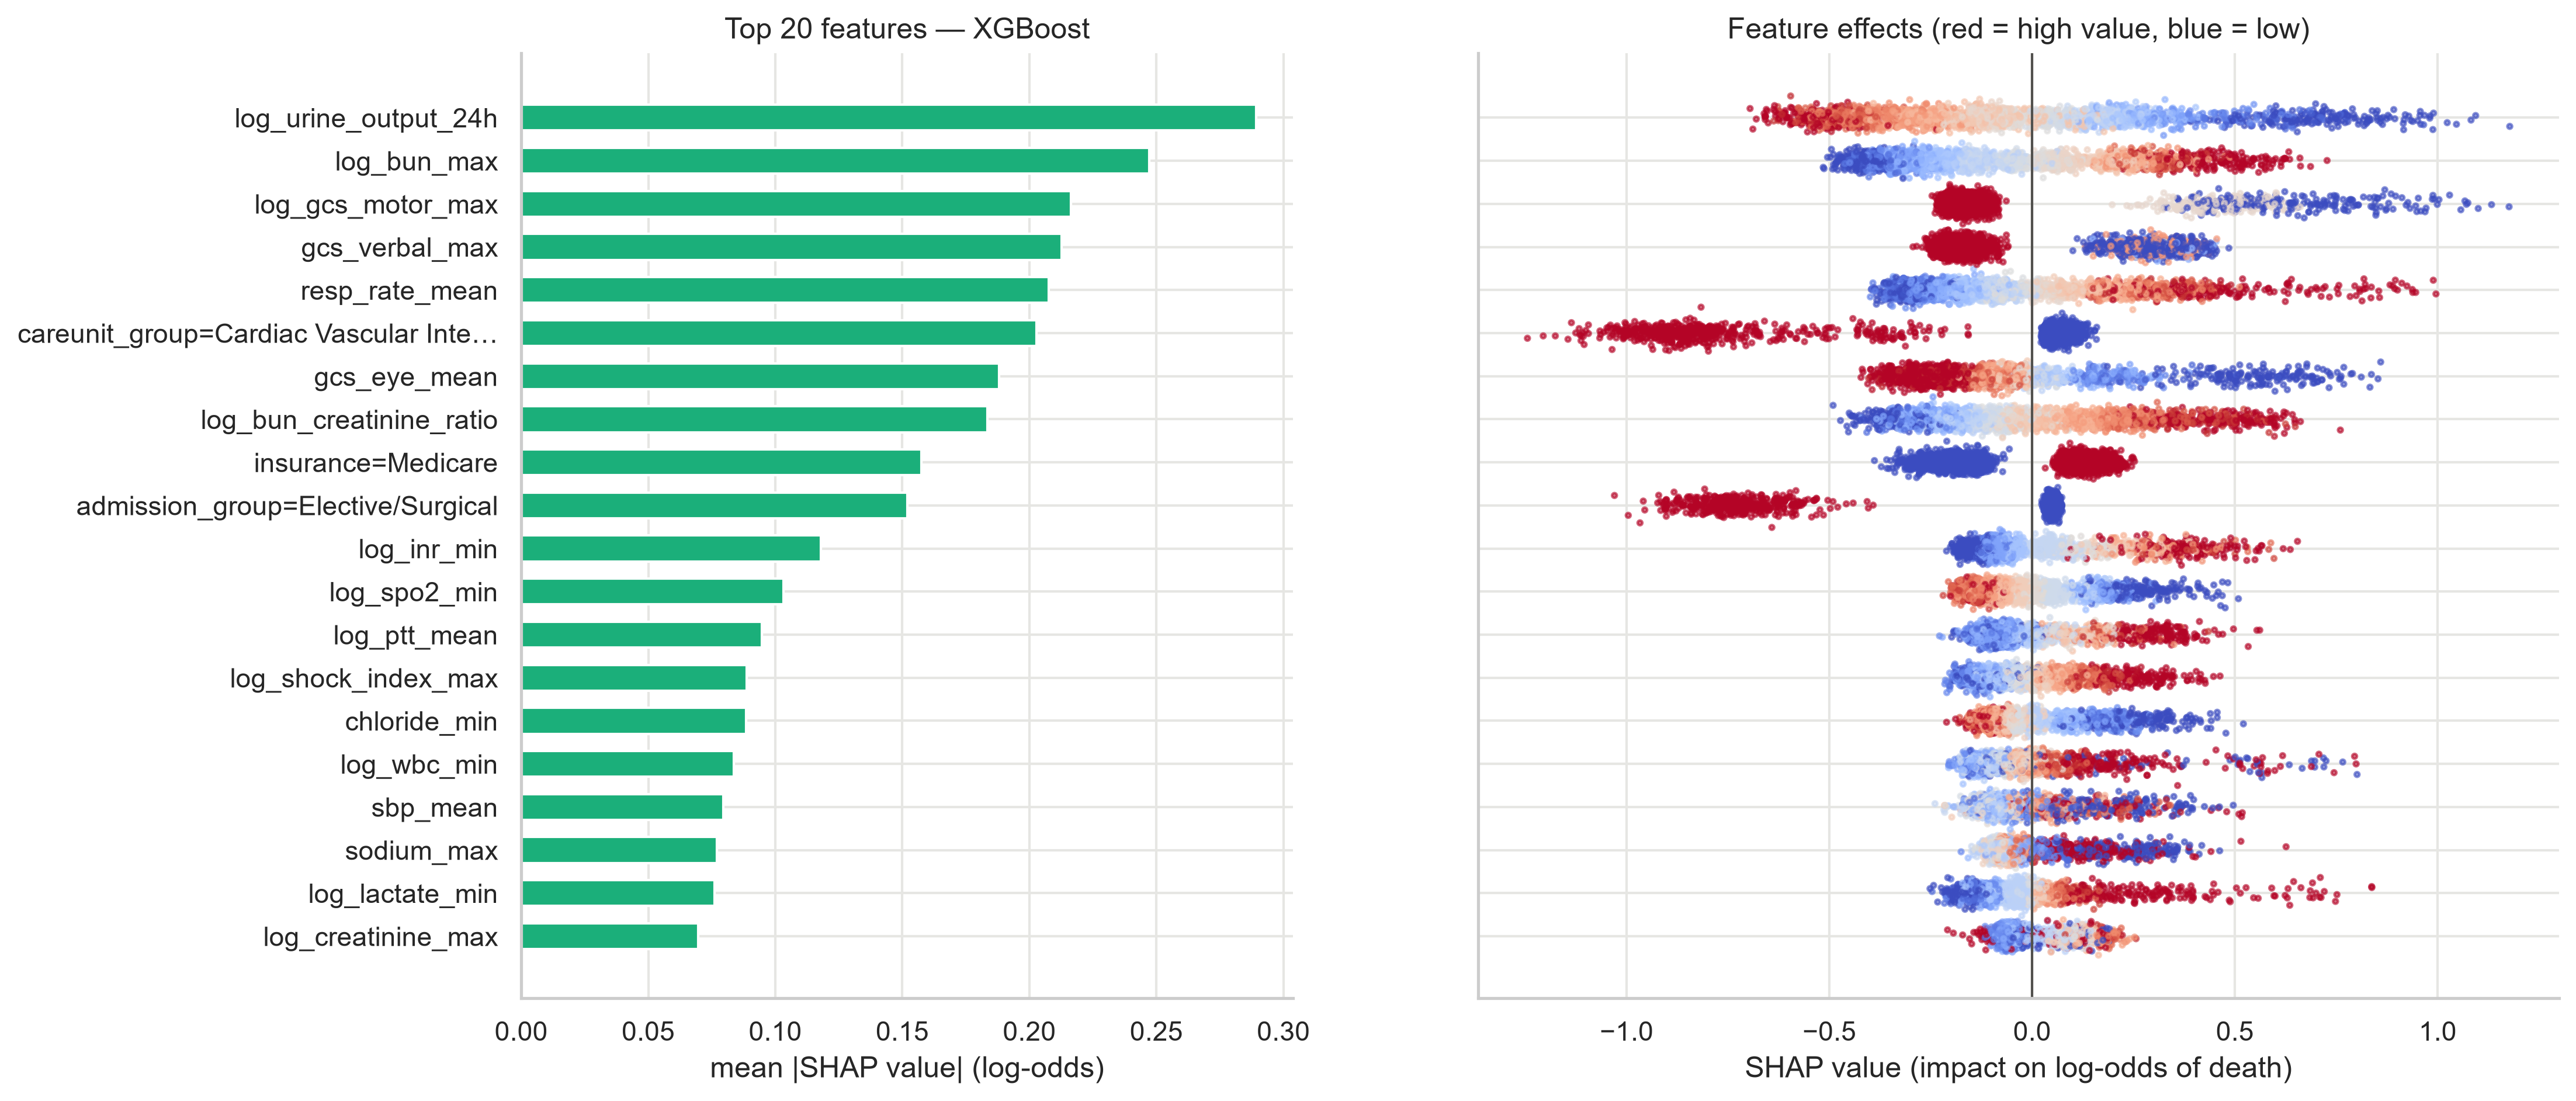
\includegraphics[width=0.92\textwidth]{fig_shap.png}
\caption{SHAP feature importance (left) and feature effects (right) for XGBoost on 3,000 test stays.}
\label{fig:shap}
\end{figure*}

\subsection{Subgroup Performance}
\TEAM{Table~\ref{tab:subgroups} and Fig.~\ref{fig:subgroups}: largest AUROC gap by age band (0.833--0.922), then
insurance (0.870--0.918) and admission period (0.873--0.918); sex (0.888--0.895) and admission type almost equal.
Name which groups have the lowest AUROC and any calibration-in-the-large gaps from the figure; mention the
unstable small groups.}

\begin{table}[!t]
\caption{Range of test-set AUROC across subgroups (groups with $\geq$100 deaths)}
\label{tab:subgroups}
\centering
\footnotesize
\begin{tabular}{@{}lrccc@{}}
\toprule
Attribute & Groups & AUROC range & Gap & Max ECE \\
\midrule
Age band & 5 & 0.833--0.922 & 0.089 & 0.020 \\
Insurance & 3 & 0.870--0.918 & 0.048 & 0.012 \\
Admission period & 5 & 0.873--0.918 & 0.045 & 0.017 \\
Care unit & 5 & 0.856--0.898 & 0.042 & 0.020 \\
Race & 2 & 0.885--0.898 & 0.013 & 0.041 \\
Sex & 2 & 0.888--0.895 & 0.007 & 0.006 \\
Admission type & 3 & 0.877--0.883 & 0.006 & 0.016 \\
\bottomrule
\end{tabular}

\end{table}

\begin{figure*}[!t]
\centering
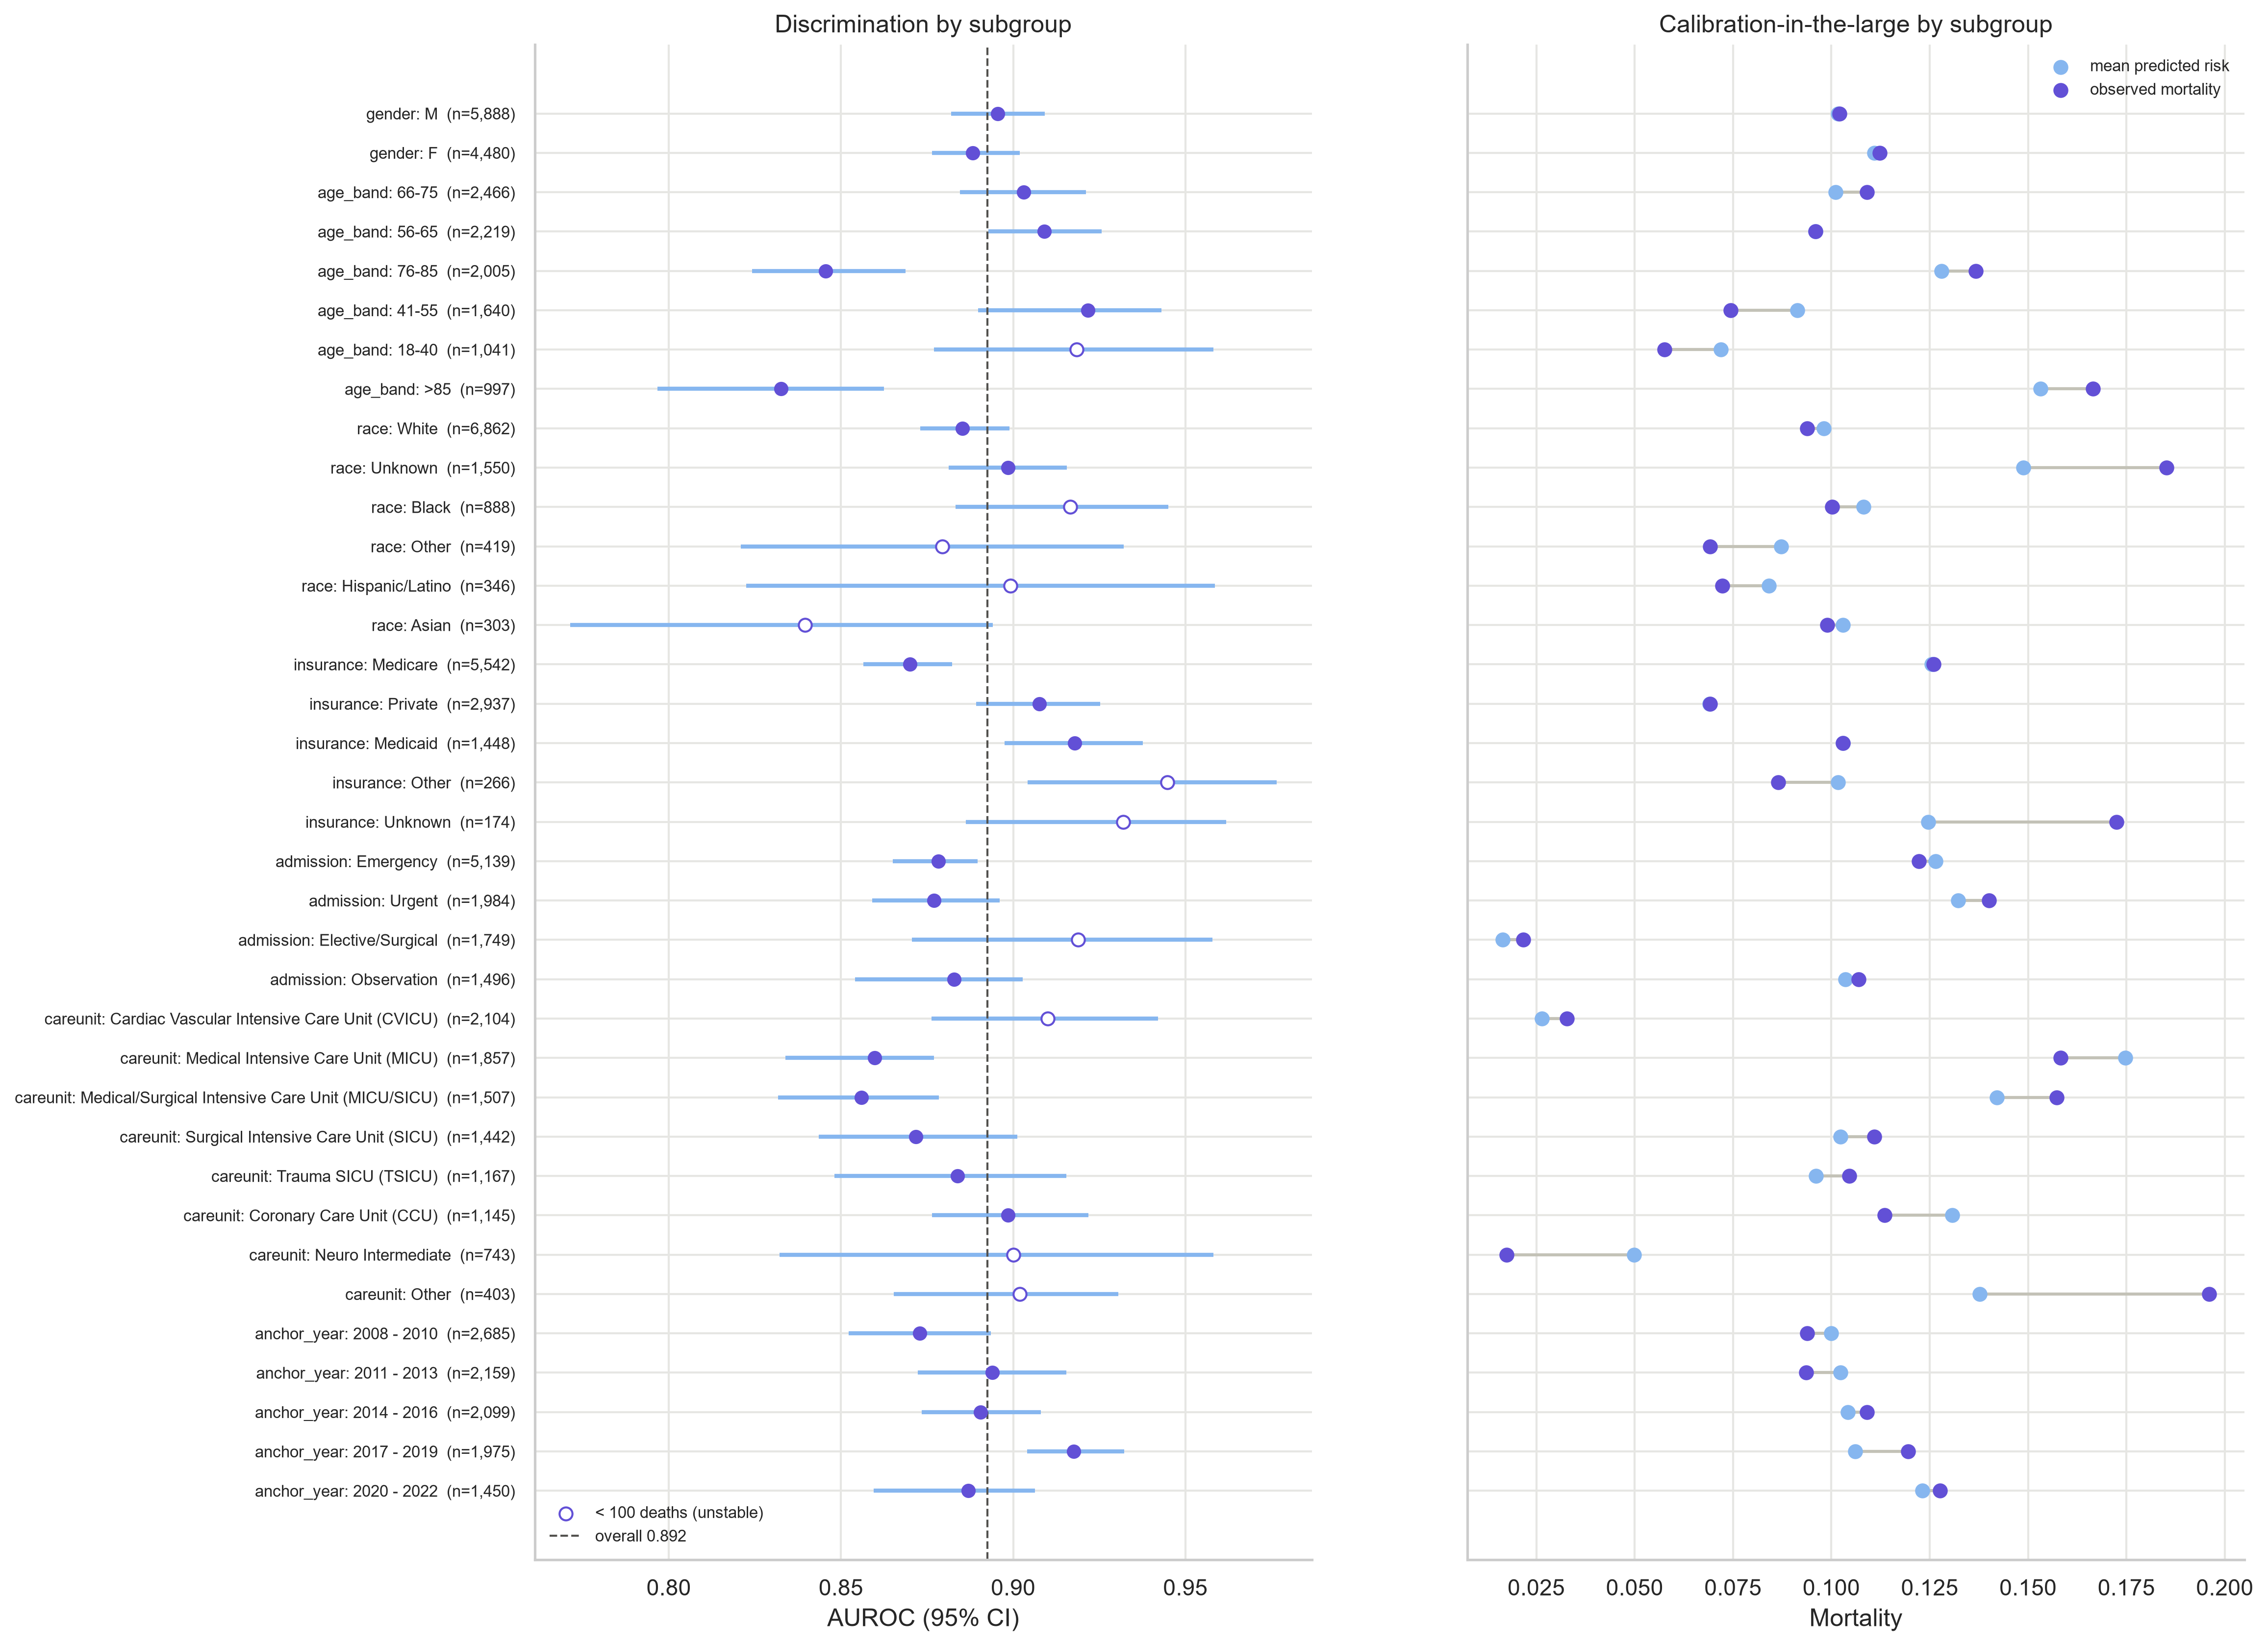
\includegraphics[width=0.95\textwidth]{fig_subgroups.png}
\caption{Subgroup AUROC with 95\% CIs (left) and observed vs. mean predicted mortality (right) for the final model.
Open markers denote subgroups with fewer than 100 deaths.}
\label{fig:subgroups}
\end{figure*}

\subsection{Missing-Data Strategies and Temporal Hold-Out}
\TEAM{Table~\ref{tab:missing} and Fig.~\ref{fig:missing}: complete-case training used only 15\% of stays and lowered
AUPRC on all test stays (logistic regression 0.437 vs. 0.471; XGBoost 0.503 vs. 0.534); the other strategies were
similar (note: only one of the 40 selected features is a missing indicator). Table~\ref{tab:temporal}: in
2020--2022, AUROC fell slightly (logistic regression 0.871$\rightarrow$0.851; XGBoost 0.890$\rightarrow$0.879) with
overlapping CIs.}

\begin{table*}[!t]
\caption{Missing-data strategies (isotonic-calibrated; CC = complete-case test subset)}
\label{tab:missing}
\centering
\footnotesize
\begin{tabular}{@{}llrrrrr@{}}
\toprule
 & & & \multicolumn{3}{c}{All test stays} & CC subset \\
\cmidrule(lr){4-6}\cmidrule(lr){7-7}
Strategy & Model & Train rows & AUROC & AUPRC & ECE & AUPRC \\
\midrule
Imputation + indicator & Logistic regression & 100\% & 0.869 & 0.471 & 0.006 & 0.597 \\
Imputation + indicator & XGBoost & 100\% & 0.890 & 0.534 & 0.002 & 0.660 \\
Median imputation only & Logistic regression & 100\% & 0.869 & 0.474 & 0.007 & 0.603 \\
Median imputation only & XGBoost & 100\% & 0.890 & 0.538 & 0.004 & 0.665 \\
Complete-case & Logistic regression & 15\% & 0.837 & 0.437 & 0.008 & 0.615 \\
Complete-case & XGBoost & 15\% & 0.873 & 0.503 & 0.003 & 0.648 \\
Native NaN (XGBoost) & XGBoost & 100\% & 0.889 & 0.532 & 0.005 & 0.663 \\
\bottomrule
\end{tabular}

\end{table*}

\begin{figure*}[!t]
\centering
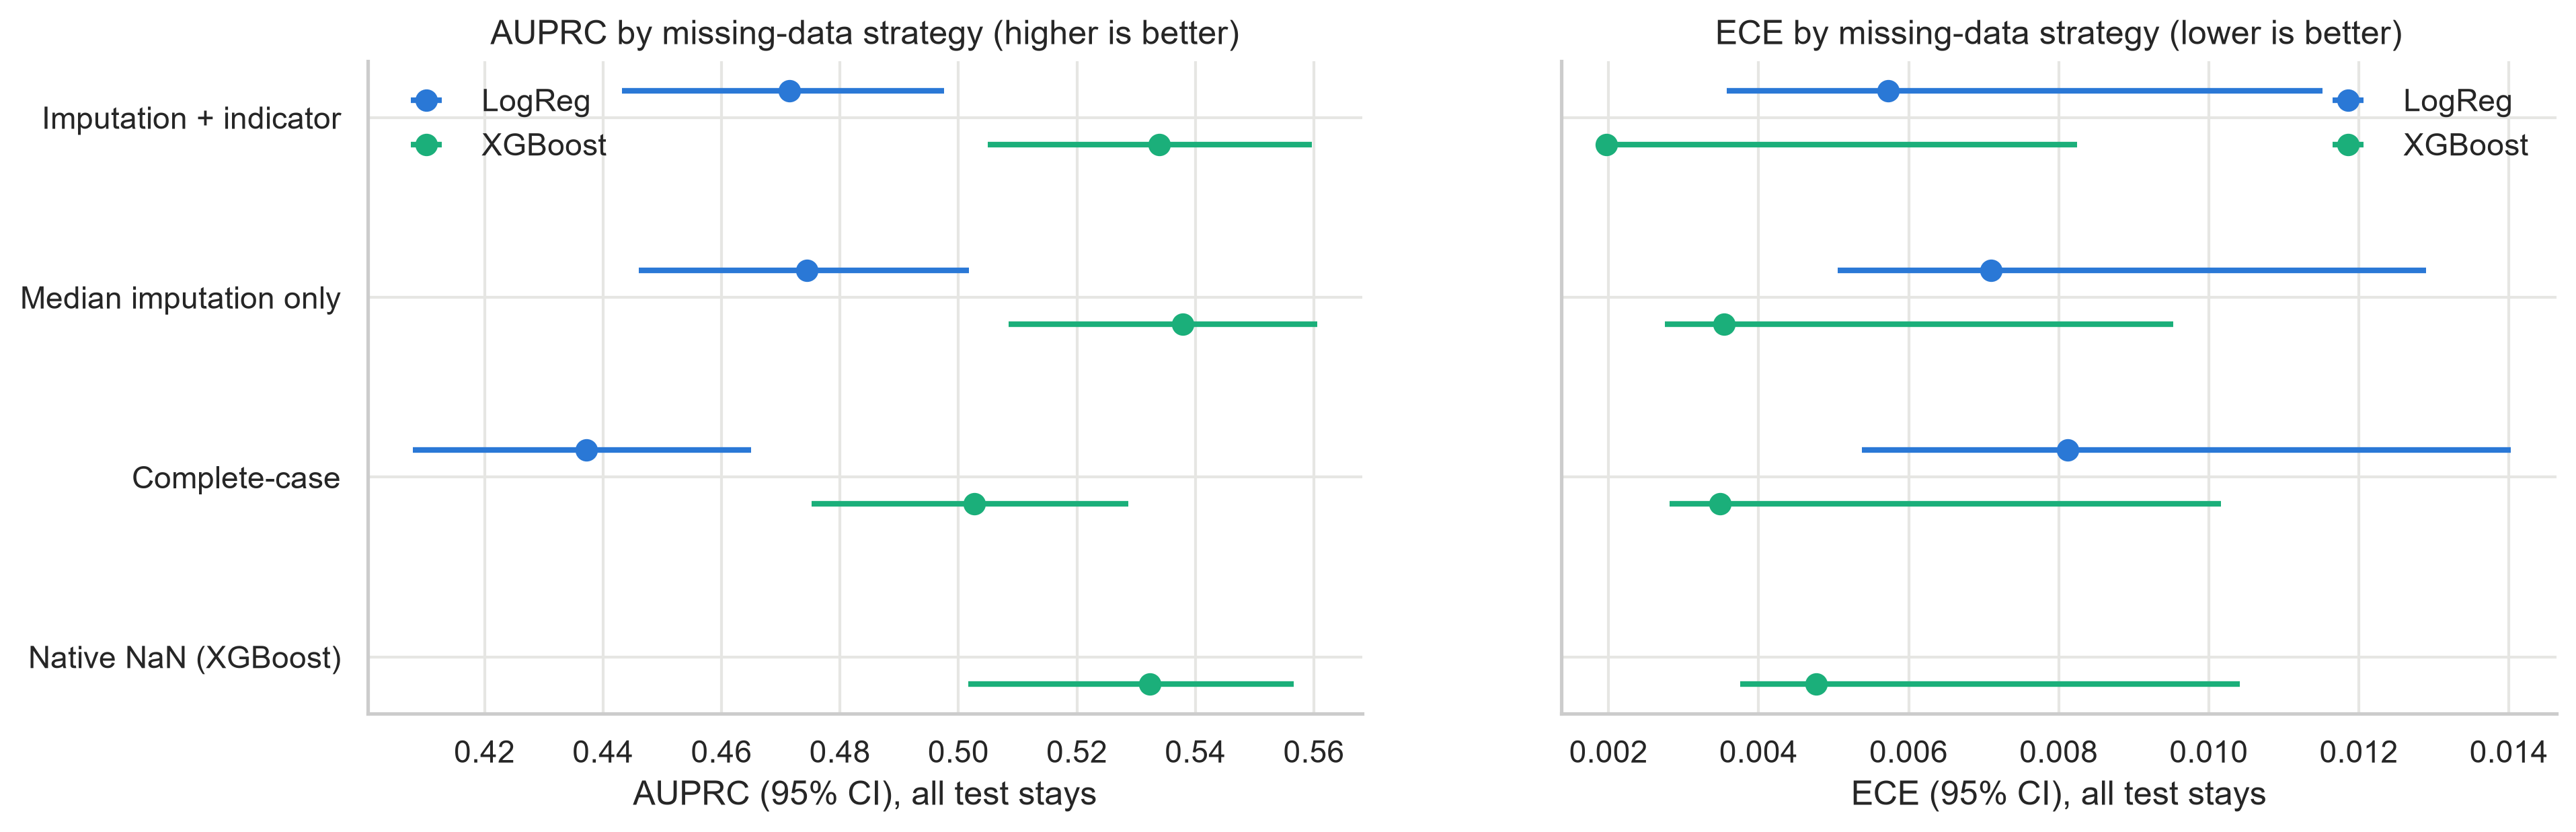
\includegraphics[width=0.85\textwidth]{fig_missing_strategies.png}
\caption{AUPRC and ECE by missing-data strategy on all test stays.}
\label{fig:missing}
\end{figure*}

\begin{table}[!t]
\caption{Temporal hold-out using admission period}
\label{tab:temporal}
\centering
\scriptsize
\setlength{\tabcolsep}{3pt}
\begin{tabular}{@{}llrcc@{}}
\toprule
Model & Test period & $n$ & AUROC & AUPRC \\
\midrule
LR & 2008--2019 & 8,918 & 0.871 (0.859--0.881) & 0.475 (0.445--0.507) \\
LR & 2020--2022 & 1,450 & 0.851 (0.816--0.881) & 0.483 (0.400--0.558) \\
XGBoost & 2008--2019 & 8,918 & 0.890 (0.878--0.901) & 0.536 (0.500--0.566) \\
XGBoost & 2020--2022 & 1,450 & 0.879 (0.849--0.902) & 0.543 (0.471--0.612) \\
\bottomrule
\end{tabular}

\end{table}

% =====================================================================================================
\section{Discussion}
\label{sec:discussion}

\TEAM{Paragraph 1 - main findings in plain words (good discrimination and near-perfect calibration after
recalibration; moderate ML gain; large gain over SOFA).}

\TEAM{Paragraph 2 - comparison with literature, carefully: e.g. MIMIC-III benchmark mortality AUROC around 0.86
\cite{harutyunyan2019multitask}; results vary with cohort definitions \cite{johnson2017reproducibility}; direct
comparison is limited because cohorts, windows and prevalence differ (AUPRC depends on prevalence). Explain why
higher published numbers can come from record-level splits, longer windows or leakage, which our design avoids.
Verify any number you quote against the paper.}

\TEAM{Paragraph 3 - H3 and calibration: relate the moderate gain to Christodoulou et al.
\cite{christodoulou2019systematic}; why reporting calibration changes conclusions \cite{vancalster2019calibration}.}

\TEAM{Paragraph 4 - missing data and subgroups: what the complete-case result means for studies that drop incomplete
patients; what the age-group gap means for deployment and fairness \cite{obermeyer2019dissecting}.}

% =====================================================================================================
\section{Limitations}
\label{sec:limits}

\TEAM{Single centre, retrospective; only a weak temporal check (dates shifted per patient) and no external validation
(e.g. eICU); SOFA without vasopressor doses; 24-h window only (protocol's 6/12-h comparison not done); reduced tuning
budget (3 folds, 6--25 trials) to fit the compute time; race and insurance are coarse administrative categories;
Part~1 preprocessing not packaged as one object.}

% =====================================================================================================
\section{Conclusion}
\label{sec:conclusion}

\TEAM{3--5 sentences: what was built, the headline numbers, the main lesson for reporting (calibration, missing
data, grouped validation, subgroups), and future work (external validation, more windows, recalibration over time).
Give the GitHub link: https://github.com/mudasarzulfiqar01/mimic-icu-mortality-calibration}

% =====================================================================================================
\section*{Acknowledgment}

\TEAM{Thank PhysioNet and the MIT Laboratory for Computational Physiology for MIMIC-IV; state that all authors
completed the required credentialing and followed the data-use agreement. If your course requires it, add an
AI-assistance statement describing honestly how AI tools were used (e.g. code, figures, tables, LaTeX template).}

% =====================================================================================================
\bibliographystyle{IEEEtran}
\bibliography{references}

\end{document}
